\chapter{Introduction to Information Retrieval}
\section{Overview about Search Engines}
Nowadays the Information Retrieval is much more than building search engines.\newline 
Altavista was the \textbf{first search engine} that has been widely used from people. It has been developed in 1993-1994.\newline
There were advertisements that nowadays are not present anymore in our search engines. Now they are more easy to use, instead during the past they were more complicated.\newline
For example there was a button "Add URL" that allowed you to add your own web page to their search engine because it was difficult to find web pages. There was even an advanced search because at that time people that were using it they were skilled. This means that they were able to make logical queries or proximity queries. In our days this doesn't happen anymore because the Web users are not so skilled. With Altavista there was only text in pages for example they totally forgot about hyperlinks.\newline
After few years (1997-1998) it came out Google. It was similar to Altavista, but it had a new "feature": they showed on the home of Google the number of indexed pages that it was 25 million of pages, then this "feature" disappeared.\newline
Google had some User Interface features like "I'm feeling lucky" (to make fun of Altavista) or a subscription and even more...
It can be looked in the image below (Figure \ref{fig:googlehomepage}).\newline \newline
\begin{figure}
    \centering
    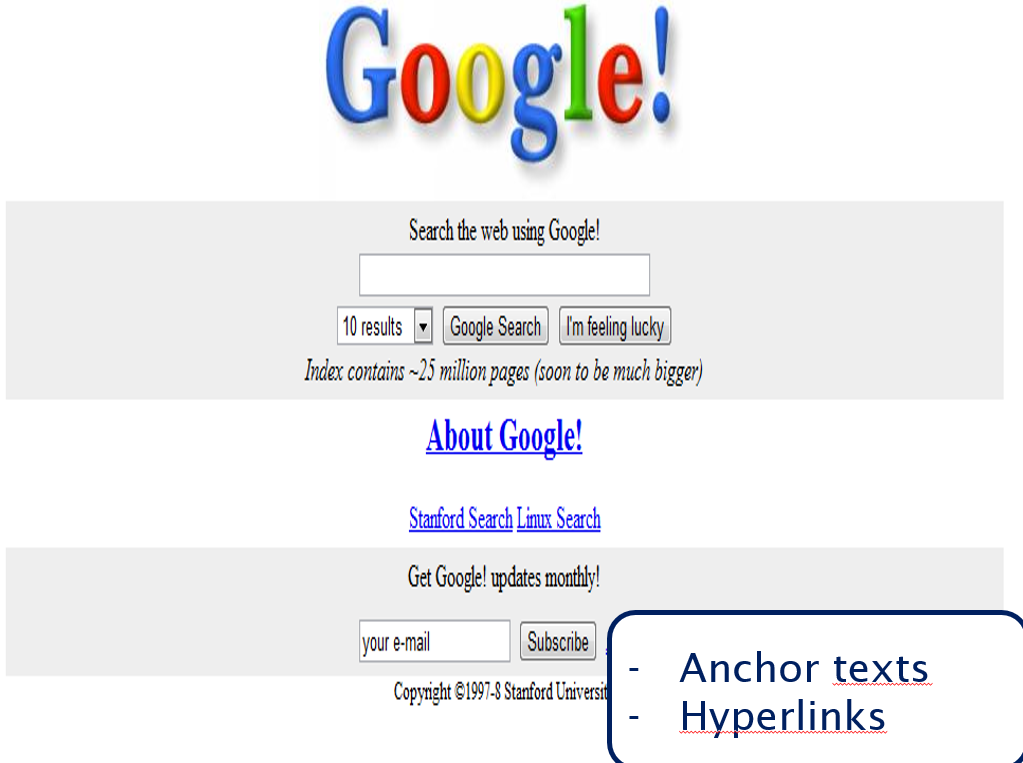
\includegraphics[width=0.65\linewidth]{images/googlehomepage.png}
    \caption{Google home page}
    \label{fig:googlehomepage}
\end{figure}
From a technical point of view there were two new things:
\begin{itemize}
    \item \textbf{Anchor text} (blue text that characterize an hyperlink); this is so important because if I look at the anchor text I can create an idea of the page where I land, so it helps me to understand what is the content of the page if I click on it; at the beginning it was so good, but unluckily the Web is not a good world (we will see later why, but remember Google bombing);
    \item \textbf{Hyperlinks} (links between pages); they allowed to create graphs where you could look at the edges between each page;
\end{itemize}
Then there was a \textbf{third generation} around 2005 and there were more sources like news, images, maps and Wikipedia. So people weren't looking only for pages but other things too, that's why pages weren't enough. This generation is known as \textbf{"multi-source"}.\newline
After few years there were only four search engines:
\begin{itemize}
    \item Google
    \item Bing
    \item Ask
    \item Yahoo!
\end{itemize}

In 2009 Ask disappeared in the sense that nowadays it exists and it works, but it can't be considered a world wide search engine due to his low percentage usage. After few years Yahoo! disappeared too in the sense that the backbone is not longer from them, but they take the results from Bing.\newline
The two biggest search engines are Google and Bing, there are even Yandex (Russian search engine) and Baidu (Chinese search engine). Their problem is that they are largely used in their countries, but around the world the usage percentage is very low.\newline
Around 2012 there was the \textbf{fourth generation} which is the current generation and it is related to different concept. Google introduced the \textbf{knowledge frame} which is a frame you find some knowledge.\newline
For example if you're looking for Galileo you will have the same page as in the past, but on the right you have a new frame that shows you some information related to your query like images, few lines of information like date of birth, written books and other stuff like that. It can be seen in the following image (Figure \ref{fig:galileo}).
\begin{figure}
    \centering
    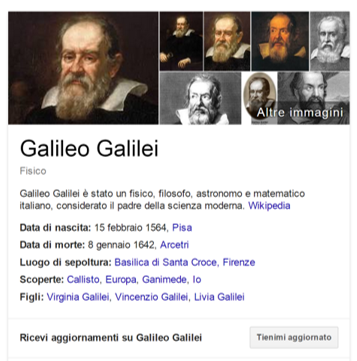
\includegraphics[width=0.55\linewidth]{images/knowledgeFrame.png}
    \caption{Knowledge frame}
    \label{fig:galileo}
\end{figure}
From this feature, people discovered that Google was using something new: \textbf{Knowledge Graph}. There are edges that encode relations between the nodes. The nodes can be people, cities, concepts, events. 
In our days this graph is huge there are billions of nodes, trillion of edges and thousands of relations between nodes.\newline
Graph algorithms are becoming crucial, they are so helpful.\newline
An example of Knowledge Graph is Wikipedia that it's a small Knowledge Graph (but not too small! In English is 6-7 million of pages). 
What is the feature of this Knowledge Graph? Every node (textual content) is a page and each node points to other nodes (anchor texts). Be careful that each anchor text is not the title of the node, for example a node can be "Diego Armando Maradona", but in other pages we can have anchor texts like "El Pibe De Oro" or "Maradona".
In the Knowledge Graph each page can be called \textbf{entity} too.
This concept is so important because suppose that we have:
\begin{quote}

\centering \textit{"Leonardo is the scientist that has painted Mona Lisa"}
\end{quote}
If our Knowledge Graph is enough developed we will have two entities (pages) that are "Leonardo da Vinci" and "Mona Lisa - painting".
This is important because all the nodes are in a graph so we can "expand" the graph and for example we will have that "Leonardo da Vinci" is linked with "Italy" or "Cartography" or "Science" that are nodes too.
The construction of Knowledge Graph depends on what is the context, for example there are some companies that are working on how to build a Knowledge Graph that it is "vertical" in the sense that it is specialized on a specific topic like Biology or Technology or Sport. On the other hand there are companies like Google that try to build Knowledge Graph for everything.
A problem to solve is that for example for "Leonardo", our system should be able to understand if "Leonardo" stands for "Da Vinci" or "Di Caprio" (if it exists).
This problem is called \textbf{polysemy} it happens when the same word has different meaning in two sentences that are similar. Look at the example below.
\begin{quote}
    \centering \textit{The paparazzi photographed the star}
\end{quote}
\begin{quote}
    \centering \textit{The astronomer photographed the star}
\end{quote}
If the algorithm that we build is "smart" it should be able to understand how much is important "paparazzi" or "astronomer" because then the meaning of "star" changes totally.
Another key point is \textbf{synonimy} and this happens when we use different words for the same concept. Look at the example below.
\begin{quote}
    \centering \textit{He is using Microsoft's browser}
\end{quote}
\begin{quote}
    \centering \textit{She plays with Internet Explorer}
\end{quote}
To solve this problem is to plug into the machine knowledge that these two different words must be mapped on the same page/node.\newline
Let's make a short resume about the evolution of Search Engines:
\begin{itemize}
    \item \textbf{Zero generation} (1991): it was the prehistory of search engines; just some metadata added by users; an example can be Wnaderer;
    \item \textbf{First generation} (1995-1997):  it used only on-pages (without anchor text); an example can be AltaVista or Excite or Lycos;
    \item \textbf{Second generation} (1998): it started to use off-page (anchor text); an example can be Google;
    \item \textbf{Third generation} known as "the need behind the query": it was focused on "user needs" rather than on query (if a page is a lot of clicked I have to take it into account) and it started to integrate multiple data-source; an example can be Google, Yahoo!, MSN or Ask; 
    \item \textbf{Fourth generation} known as "Information Supply" (current): it is used this description because it often happens that people write just one term in the query that's why you can't understand the user needs and for this reason you show to the user different "categories" like news, images and so on; otherwise if you have the profile of the user you can use his information to be more precise;
\end{itemize}
\subsection{What is the Paradigm Shift?}
To understand better how nowadays Search Engines work we have to talk about a \textbf{Paradigm Shift} that it is something more complicated that involves Computer Science because the search engines are part of this world.
Now we have <<devices 2.0>> that have their ID, Communication capacity, computing and storage and currently interaction ability and they work with Search Engines.
There are devices that "sensing" taking data from the world and then there are algorithm that "actuating" actions in the real world (IoT stuff).
Just to have an idea top level cars like Tesla have an interface that can access to Internet and navigate the Internet, this changed the interaction with search engine. For example now we have a voice interaction like Siri or Google Now. These tools changed the Web Engine because in the past when we people typed queries they were so lazy, they typed just 2-3 words for a query; now that there is a voice interaction people talk a lot and the queries are long (classic interaction of humans).
The "loop" changed because in the past the humans were obviously in the loop, but now the humans don't have to be inside the loop like IoT where devices answer to other devices.
If there is an interaction between two devices instead of human-device there are some things that change. For example we are able to look few results like 7-10 pages instead a device is able to look at thousands of pages.\newline
\subsection{Three types of data}
There are three main types of data:
\begin{itemize}
    \item \textbf{Opportunistic}: it is used this term because people are using something like credit card or telephone calls, but the result is that there are companies that take this data and use them in an opportunistic way for other stuff like finding friends in order to promote some advertisement;
    \item \textbf{Purposely sensed}: it is the typical pollution, temperature, movement; they are typical data used for something really specific;
    \item \textbf{User generated}: you ask people to contribute; this is typical social networks where you post photos or tweet;
\end{itemize}
Notice that the same data can be used for different purposes for example if there are some sensors that count each car that cross the street can be used either as purposely sensed either in an opportunistic way.\newline
Notice that search engines are not only things like Google, but even TomTom is a search engine where your query is a specific city or address (\textbf{searching routes}).
Even TripAdvisor is a search engine and you are not only searching by text, but even by distance so you have to take into account geography (\textbf{searching over Geo + labels}).\newline
Linkedin too is an information retrieval tool (\textbf{searching over labeled graphs}) where people are nodes and edges are connections between people.\newline
\newline
\section{Basics of Information Retrieval}
Now we start from a techincal point of view.
\subsection{Definition of Information Retrieval}
What is the definition of Information Retrieval? \textbf{Information Retrieval} (IR) is \textbf{finding material} (usually documents) of unstructured nature (usually text) that satisfies an \textbf{information need} from within \textbf{large collections} (usually stored on computers).
\subsection{Structured data vs. Unstructured data}
Usually we don't speak of Databases because they are table and they refer to \textbf{structured data} and the query is exact specified without ambiguity. In search engine we don't have this kind of query and the results aren't something really specific, but they are something that remind to your query (all the expressions that aren't well defined from a mathematical point of view).\newline
In our case we have \textbf{semi-structured data} like XML or JSON, we look the data as trees. To be honest almost no data is "unstructured" for example a slide has different zones like \textit{Title} or \textit{Bullets} and you can use operators like "contains".
Of course there are some issues like: "how do your process operator "about"?" or "how do you rank results?".\newline
At the end we have \textbf{unstructured data} that typically refers to free text and allows keyword queries including operators and there are some concept more sophisticated like "find all the web pages dealing with drug abuse".
\subsection{Boolean queries}
In search engine we have also \textbf{Boolean queries} because we have also the connector in the query. For example if I am looking for "Paolo Ferragina" implicitly I'm looking for "Paolo" AND "Ferragina", but the AND it's not an \textbf{Hard-AND}, it is a \textbf{Soft-AND}.\newline
If I search something on Google using two words that are too specific then Google "remove" one of them to relax the constraints.\newline
This search system is still used by Email, library catalog or Mac OS X Spotlight.\newline
Now let's go more in details why didn't the creator of Google used known structures like databases? To understand this let's look at an example.
Suppose that we want to build a search engine for Shakespeare poems, in the column we put the poems of Shakespeare (suppose that they are six) and on the rows we put the words that appear in each poem.\newline
Let's look at the following image (Figure \ref{fig:booleanmodel}).
\begin{figure}
    \centering
    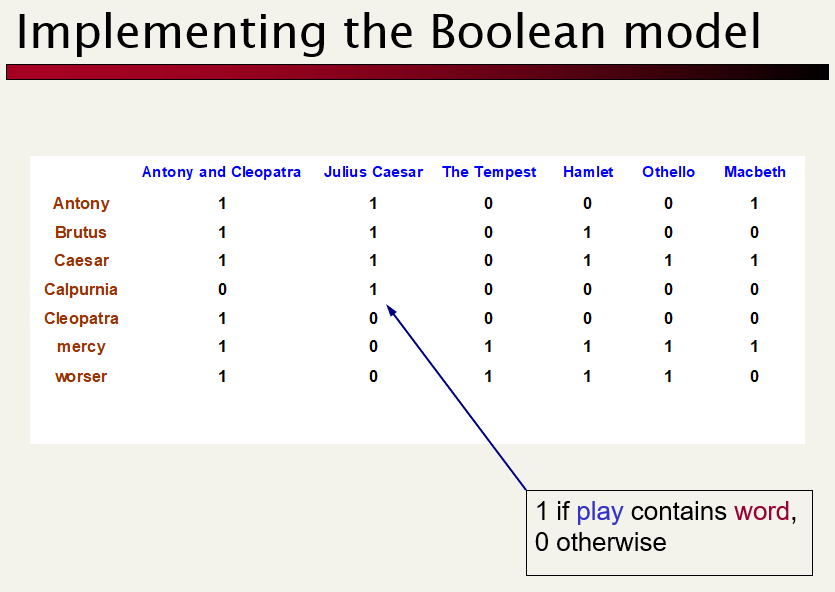
\includegraphics[width=0.8\linewidth]{images/boolean model.png}
    \caption{Implementing the Boolean model}
    \label{fig:booleanmodel}
\end{figure}
Now assume that the query is "Anthony AND Brutus", I have to find all the documents that contain Anthony and Brutus taking the two rows and doing a logical AND between them and if I get 1 I take the corresponding column otherwise I discard it.\newline
The problem of this approach is that there is a space problem because there are a lot of redundant zeros, this means that the matrix will be significant sparse. 
For example if I look at English Wikipedia there are over than 1 millions of pages (columns) and over 1 million of words (rows). If I create a matrix this matrix will be a matrix of size 1 million x 1 million and most of the cells will be sparse.\newline
Something different must be done: the data structure \textbf{inverted index} or \textbf{posting list}. For each term t (they are called \textbf{tokens}, sequence of character and numbers), we must store a list of all documents that contain t. We identify each document by a docID, a document serial number, like in the following image (Figure \ref{fig:inverted}). 
\begin{figure}
    \centering
    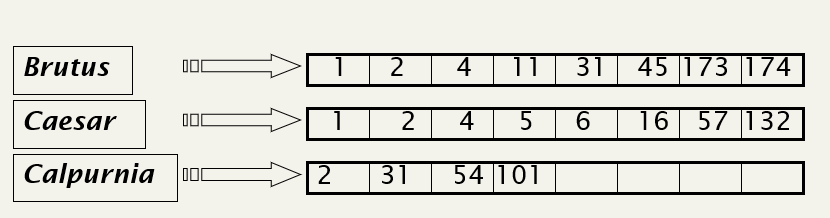
\includegraphics[width=0.75\linewidth]{images/invertedindex.png}
    \caption{Inverted index.}
    \label{fig:inverted}
\end{figure}
What happens if I want to insert a new docID? I just need to assign to it a docID then I need to scan it and looking the words, for each of them I go into the dictionary and if the term is new I add it to the dictionary otherwise I access to the list and put the docID (at the end obviously). Remember that the inverted index is ordered.
How do we solve an AND query? And why do I need to keep the lists sorted? If the lists are not sorted and I want to make an AND query between two lists, I need to start from the first one and for each element inside the first list I need to check ALL the elements of the second list. What is the complexity? If n and m are the lengths of the lists, I need to do n*m comparisons.\newline
If we sort the list it is easy and faster than the first solution. The algorithm works similar to merge in the Merge Sort algorithm. They start from the beginning and if they are equal I found a solution otherwise I let to advance the smallest one to the next position. I do this until I reach the end. In this case the number of comparison is equals to n+m. Obviously here it's better we do (n+m) comparisons instead of (n*m).
You can see the pseudo code in the following figure (Figure \ref{fig:pseudocode1}).
\begin{figure}
    \centering
    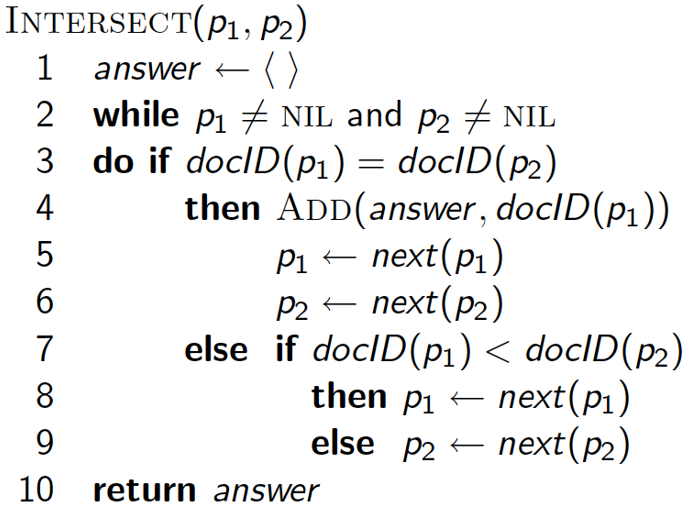
\includegraphics[width=0.75\linewidth]{images/intersectpseudo.png}
    \caption{Pseudo code}
    \label{fig:pseudocode1}
\end{figure}
At the end we can highlight two advantages of the sorting:
\begin{itemize}
    \item \textbf{Speed}: query requires just a scan;
    \item \textbf{Space}: store smaller integers thanks to the gap coding; Compressed they occupy 1-3 \% of original text;
\end{itemize}
What happens if the user specify more than two terms, but for example n tokens? What is the best order for query optimization? First of all for each of the n terms, get its postings lists, then AND them together. How do we choose the order? It is better to choose the shortest two, make the AND between them and so on.
For example look at the following image (Figure \ref{fig:optimization}), it is better to make the AND between Calpurnia and Brutus and the result with Caesar because they are the shortest two so it will happen that they can share at most two items (Calpurnia has length two and Brutus has length seven). Doing this I can optimize my space because the result will be shorter.
\begin{figure}
    \centering
    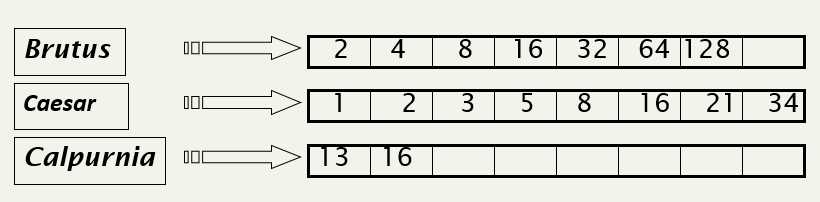
\includegraphics[width=0.75\linewidth]{images/optimization.png}
    \caption{How to process a query with n tokens?}
    \label{fig:optimization}
\end{figure}
We should highlight that the algorithm depends on the lists because the algorithm that we have seen in the figure \ref{fig:pseudocode1} it is not the best one in this case where we have a very long list and a very short list. It would be much better to do a binary search for each item of Calpurnia since it has a very short length. Otherwise I can process at the same time n lists, I just apply the algorithm that we have seen \ref{fig:pseudocode1}, but with n index. So we have seen different solutions with different performance (three possible solutions + the one with min heap where we store the min value with the index position).
\subsection{Optimizing queries}
Another question that we can make to ourselves is: Can we improve the scanning-based intersection? We have the skips and the recursive merge.\newline
The first idea that we can apply is the \textbf{skip pointers}. For every list we keep some extra information (we occupy more space). We divide the list into logical blocks, they don't exist they are just in our mind, each head of each block has a skip pointer to the head of the next block. There is an example in the following image (Figure \ref{fig:skip}).
\begin{figure}
    \centering
    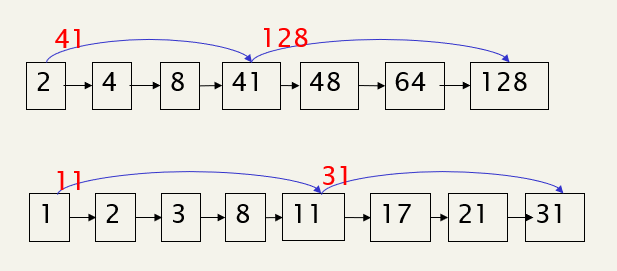
\includegraphics{images/skip.png}
    \caption{Skip pointers}
    \label{fig:skip}
\end{figure}
With a long block size I store less skip pointers and I save more space, instead with more skip pointers I save less space and obviously in the first case I have less probability to jump during scanning-based intersection, but if I do it I jump a lot of items. Otherwise in the second case I have more probability to jump, but I will jump fewer items. Usually the size of the block is chosen as if the size of the list is \textit{l} then the size of the block should be \textit{sqrt(l)}. If we know the distribution of the lists, that it's called \textbf{distribution aware}, we can change the size of the block list and the size has not to be the same for all the blocks it can change.\newline
Another way to optimize the query instead of skip pointers is the \textbf{recursive merge} without using pointers, but using pivots. It's called recursive merge for historical reasons, but the operation that it does is the intersection.\newline
Suppose that we have two lists and one of them is very short while the other one is longer. First of all we pick the median element (the one in the middle) from the shortest list and then we do binary search in the longer list. In the longer list can happen two things:
\begin{itemize}
    \item There is a match doing binary search;
    \item There isn't a match doing binary search;
\end{itemize}
In both the cases the binary search will return me a position, even if there isn't a match. Now I have that the two lists have been "splitted" in two parts and I can apply the same reason as before but for example if I am searching for the left element of the shortest list when I will do the binary search in the longer list I will do binary search with ranges [first position, position that returned me the iteration of before] because I am sure that after that position all the numbers are larger than my median element of the previous iteration.
In the following images it has been shown an example (Figure \ref{fig:recursivemerge}).
\begin{figure}
    \centering
    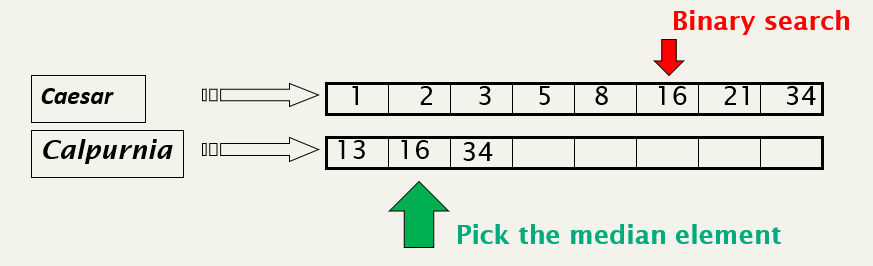
\includegraphics[width=0.75\linewidth]{images/recursivemerge.png}
    \caption{Recursive Merge}
    \label{fig:recursivemerge}
\end{figure}
This algorithm is very smart and if the median goes outside the last position of the longer list all the right part of the shortest list is removed. For example if 16 is greater than 34 then we can discard all the right part of the shortest list.\newline
What are the performance of this algorithm? If median is always out we have \textit{O(log m * log n)}. Every search takes \textit{log n} time, but I do this \textit{log m} times. We have to say that in practice this doesn't occur that's why we can't do an exact estimation of this algorithm easily.\newline
The worst case is that the median is always in the middle and the recursive relation is: \textit{T(n,m)=O(log n) + 2 T(n/2, m/2)}. This algorithm from a theoretical point of view is very elegant, but in practice is not used because it is based on recursion and it's very heavy for the machines to do that; in practice they use skip pointers.
\subsection{Queries with NOT or OR}
Until this moment we have only considered boolean queries with AND, but what happens if I want to computer NOT or OR? \newline
What is the result doing \textit{Brutus AND NOT Caesar}? When the two indexes are different then they are considered as a result otherwise if for example the min of the list 1 is equals to the min of the list 2 then I must not consider that docID.\newline
What is the result doing \textit{Brutus OR NOT Caesar}? In the case we have only OR we pick the docID in every case either if they are equal either if they are different. In this case we don't have only OR, but we have even NOT and here the situation is different. We should first of all consider \textit{NOT Caesar} that it is an huge list it will be very very long. This is not a nice query because we are "merging" a normal list ("Brutus") with an huge list that it is "NOT Caesar".\newline
Be careful that the NOT it is bad only with OR, but with AND it's not so bad.
\subsection{Different types of queries}
There are other types of queries in IR like:
\begin{itemize}
    \item \textbf{Phrasal queries} are queries like "Stanford University" (the quotes are included in the query); I expect to find out all the documents such that contain these two words one after the other one so I have to change my postings list because the structure that we have seen before doesn't work in this case;
    \item \textbf{Proximity queries} are queries like "Find Gates NEAR Microsoft"; I expect to find out all the documents such that contain "Gates" and "Microsoft" near possibly in a certain window of a certain size, for example windows\_size=3;
    \item \textbf{Zones/Fields queries} are queries like "Find documents with (author=Ullman) AND (text contains automata)"; 
    \item \textbf{Similarities queries} are queries like "Maradona", but I expect to find also "el pibe de oro"; these are queries where I check similarities among different tokens; in this case you need Knowledge Graph to make similarity checks;
\end{itemize}
To solve \textbf{Zone/Fields queries} we need first of all to define what is a zone. A zone is a region of the document that can contain an arbitrary amount of text (title, abstract, references). To do this we can build inverted indexes on fields AND zones to allow querying.\newline
There are two approaches:
\begin{enumerate}
    \item Build a posting list for each zone so I encode zones in dictionary; This one is the most used and it's very efficient;
    \item Build the posting list in a different way; the elements of the list are composed by the docID and the position where it occurs; in this case all the algorithms that we have seen don't work anymore because for example compression doesn't work anymore;
\end{enumerate}
In the following figure it has been shown an example (Figure \ref{fig:zonequeries}).
\begin{figure}
    \centering
    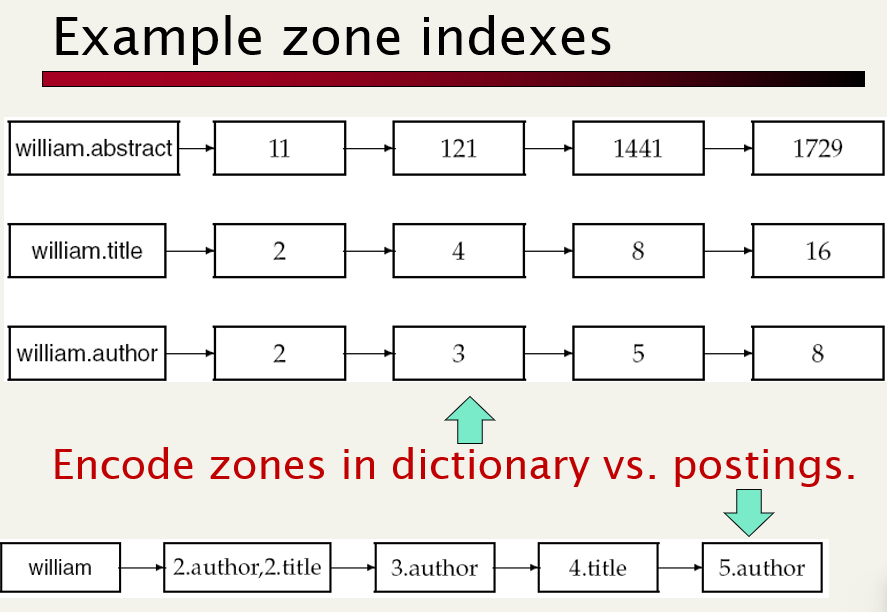
\includegraphics[width=0.75\linewidth]{images/zonequeries.png}
    \caption{Encode zones in dictionary vs. Postings}
    \label{fig:zonequeries}
\end{figure}
We are always talking on how to make queries and so on, but it's missing an entire world that it's the ranking search results. Boolean queries give inclusion or exclusion of documents, but often results are too many and we need to rank results. To rank results we can use: classification, clustering, summarization, text mining and etc.\newline
A lot of AI and Machine Learning on several kinds of features extracted from pages content and the Web for results selection and ranking.
\chapter{Structure of Search Engine}
In the following figure (Figure \ref{fig:searchengine}) it has been shown the structure of the Search Engine and all the main topics of this course.
\begin{figure}
    \centering
    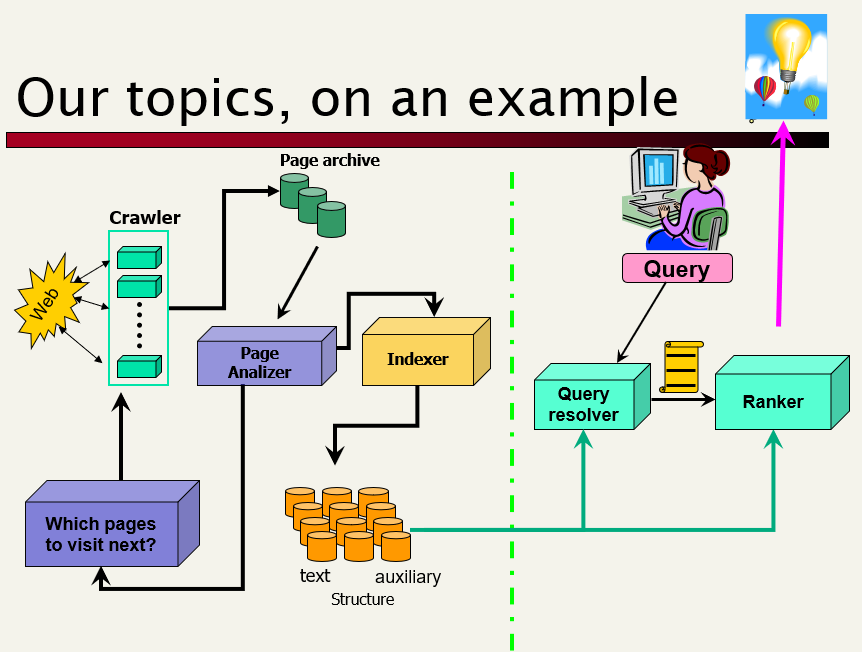
\includegraphics[width=0.85\linewidth]{images/search.png}
    \caption{Structure of Search Engine}
    \label{fig:searchengine}
\end{figure}
From the image we can see the \textbf{crawlers} that go around the Web and pick the documents. These documents are stored in a \textbf{Page Archive} and then they are analyzed because we have to build the dictionary. After that I have \textbf{parsed} the documents I have to \textbf{index} them (I have to build the inverted index that allows me to search faster). All these information are stored in an \textbf{archive} (WE ARE NOT TALKING ABOUT DATABASES). These things described are the "back-end" of the Search Engines that work 24 hours per day.\newline
On the other hand we have the "front-end" which is the part that you know. Whenever you issue a query the system gets your query and try to solve it and it solves the query accessing the index that the search engine has built. After this you have your documents and you sort them by relevance. At the end for example you show the first ten documents.\newline
In the next figure it has been shown many techniques that we will use to understand each element that we have just shown (Figure \ref{fig:functionssearch}).
\begin{figure}
    \centering
    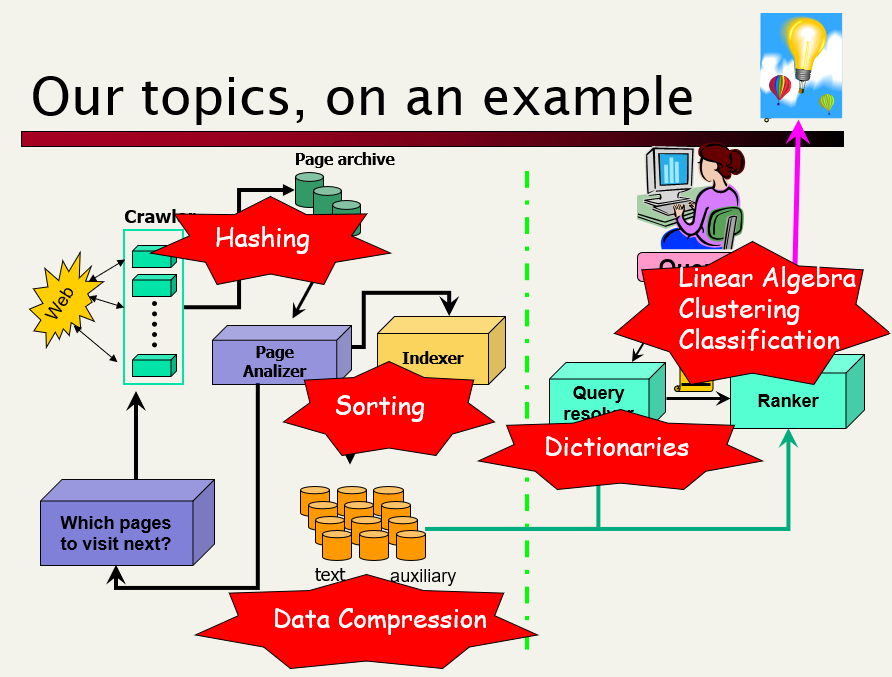
\includegraphics[width=0.75\linewidth]{images/functionsearchengine.png}
    \caption{Structure of Search Engine with functions}
    \label{fig:functionssearch}
\end{figure}
Let's give some facts in general. Let's describe the concept of "BigTable" it was very popular in 2006, but it was much older. In 2006 Google just shared it to the world and it's known as NoSQL Database that it's not a database. It's an huge table that you index by strings. You have strings on rows and columns. It's assumed to be an infinite table where you can do as operations put and get. The power of BigTable is that it's scalable, fault tolerance, secure, transactional and distributed geographically. In the following image it has been shown how it is (Figure \ref{fig:bigtable}).
\begin{figure}
    \centering
    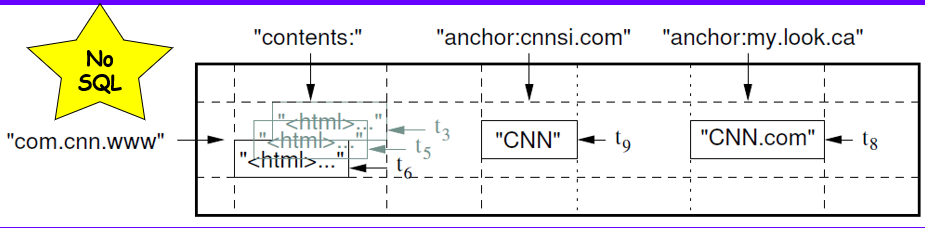
\includegraphics[width=0.75\linewidth]{images/nosql.png}
    \caption{BigTable}
    \label{fig:bigtable}
\end{figure}
Before that we go into the details we need to discuss about the Web in general. The Web has a very large size more than 1 trillion of pages, but nobody knows the real size that's why people talk about the size that it is indexed, but not the real size.\newline
The problem is that the Web is very dynamic because it changes always, it has been shown that only one third of the Web pages survive each year and only 20 \% of them are untouched, the others are always in changing. That's why extracting data from the Web is very difficult, then there are users and is difficult to match the "users needs" because 85 \% of the users look at only the first page of results that's why we must be very precise such that the first page of the results contains the right information.\newline
The Web is a graph whose size is 1 trillion of pages that each page has a size of 50-40k.
\section{Bow Tie Graph}
People think that the Web structure is \textbf{Bow Tie} and it is shown in the following figure (Figure \ref{fig:bowtie}).
\begin{figure}
    \centering
    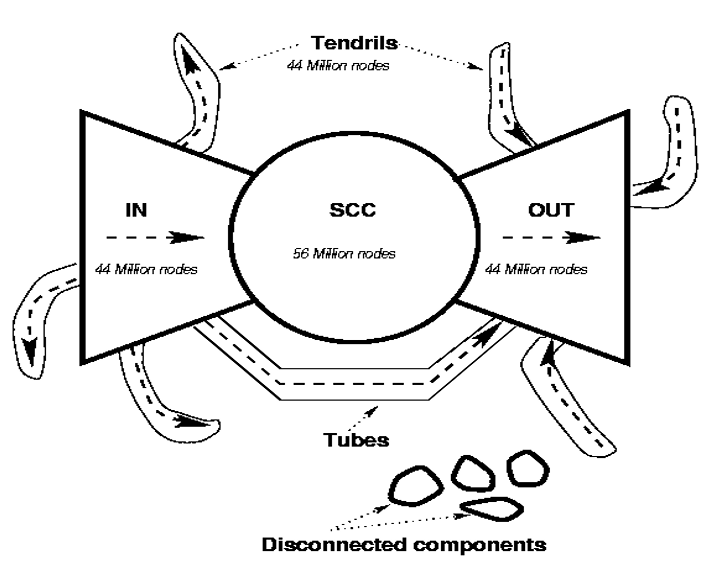
\includegraphics[width=0.75\linewidth]{images/bowtie.png}
    \caption{The Bow Tie - Structure of the Web}
    \label{fig:bowtie}
\end{figure}
The Bow Tie has different components:
\begin{enumerate}
    \item \textbf{Disconnected components}: they are part of the Web that are unreachable because they are not connected with other parts and typically they aren't interesting (if they are disconnected who cares about them);
    \item \textbf{SCC - Strongly Connected Component} (core): is a part of the directed graph, but this means that if you pick two nodes inside this component you can go from one node to the other and come back, so every pair of nodes is connected, "they are in a cycle"; this connected component is huge in the past was 56 million of nodes, now is much more bigger; one fourth of the Web is in this strongly connected component; there are other strongly connected components but they are smaller, this one is the bigger one;
    \item \textbf{IN - Connected Components}: is a part of the graph and if you pick a node inside this component you can go, through some paths, to other node always in IN or you can reach SCC; it had in the past around 44 million of nodes; remember that this has a lot of strongly connected components;
    \item \textbf{OUT - Connected Components}: is a part of the graph and if you pick a node inside this component it can be reached, through some paths, from other nodes always in OUT or nodes from SCC; it had in the past around 44 million of nodes; remember that this has a lot of strongly connected components;
    \item \textbf{Tubes}: they are sequences of pages or strongly connected components that allow you to move from IN to the OUT skipping the SCC; \textbf{remember that you can't have a path from OUT to the IN otherwise we would have an huge cycle and it would be SCC};
    \item \textbf{Tendrils}: they are sequences of pages that go from OUT or IN in some way, but they don't come back; for example it is a sequence of pages that go to my website and if in my website I don't have any hyperlink it will be stopped there;
\end{enumerate}
If I want to build a crawler it's clear that I have to start from a page that it's inside the IN component. In average these components (SCC, INN, OUT, Tubes + Tendrils) are each of them one fourth of the Web. Ideally I could take randomly four pages and one of them should stay in the IN component, but we can't do this because names aren't equally distributed. That's why people usually start from pages in the core and from them they try to reach pages from the other components.
\section{Crawling}
There are different synonyms of crawling, that's why we can hear even \textbf{spidering} or \textbf{bots} or \textit{downloader}. In few words they are programs/softwares/modules that go around in the Web and take pages (grab pages from the Web and bring them in Archive).\newline
To understand better how spidering works let's recall some notions like that the Web is a directed graph G=(N,E) where N are the nodes (pages), trillion of nodes, and E are the directed edges (hyperlinks between documents).\newline
There are some crawling issues:
\begin{itemize}
    \item \textbf{How to crawl?} we have to consider the \textit{quality} of pages, this means that we want to crawl first the "best" pages (best depends on the kind of search engine that we want to build, for example sports, news or general search engine); another key point to consider is \textit{efficiency} that's why we want to avoid duplication or near duplication in order to save space and time; we have to consider even the \textit{etiquette}, this means that the crawler has to satisfy some properties of the Web for example that he can't query many times the same server (it must not overload the server) or there are some directories that have not to be taken into account during the crawling. For this reason there is a specific file \textit{Robots.txt} that every crawler has to take into account when he acts; the last key point to consider is \textit{malicious pages} that can be divided in two different types: spam pages (offensive pages that the search engine doesn't want to crawl or not interesting pages) and spider traps (the crawler enter in these pages and start to waste time in useless pages)
    \item \textbf{How much to crawl?} we want a balance between new pages and pages that we have already seen, but we have to refresh them because these pages change like newspaper or social network; other two key points are the \textit{coverage} and \textit{relative coverage} because we know that the Web is huge and we can't cover all the pages and we can't spend time in refreshing pages that's why there is a trade-off between new pages vs. refresh pages;
    \item \textbf{How often to crawl?} the key points in this case are the \textit{freshness} and the \textit{frequency}; this issue decides how much frequent we have to come back to every page and it depends on the page because a newspaper need to be refreshed several times during the day while an university page doesn't need to be refreshed many times during the day;
\end{itemize}
In the following figure we describe what crawler does (Figure \ref{fig:crawlingexecution}).
\begin{figure}
    \centering
    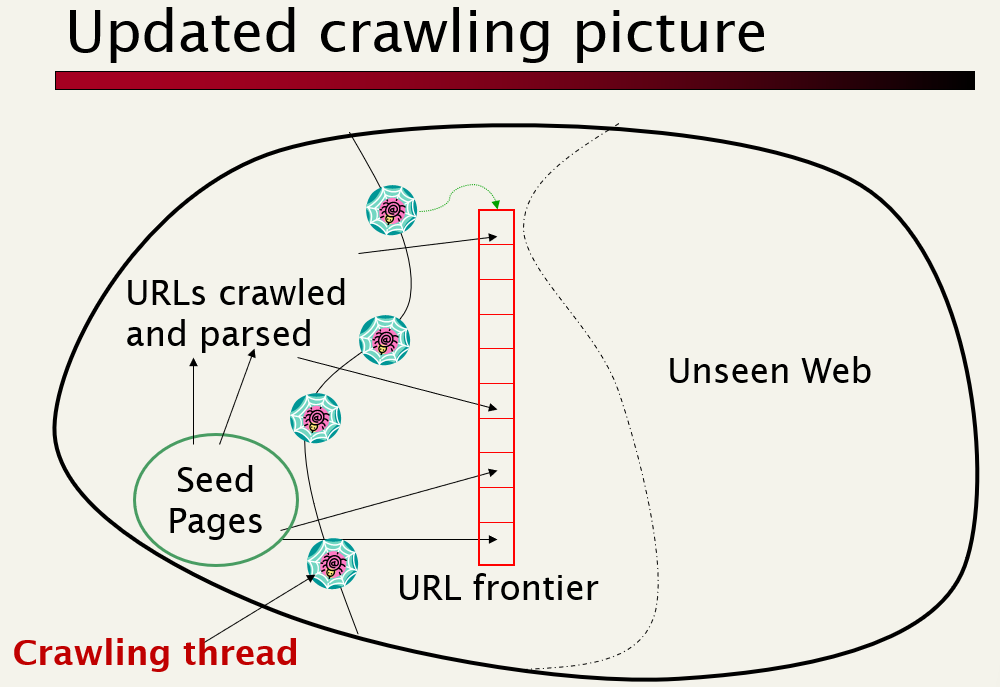
\includegraphics[width=0.75\linewidth]{images/crawlingpicture.png}
    \caption{Crawling execution}
    \label{fig:crawlingexecution}
\end{figure}
The crawler starts from a \textit{seed page} and his goal is to explore the Web graph. At a generic step we have some pages that are already crawled and are already been parsed and saved. At each step we have the \textit{URLs frontier} (it's a queue) that are URLs pointed from URLs already crawled and parsed, in other words are the set of pages that still have to be crawled. Be careful that not all the link of the URLs crawled and parsed go outside, but we can have links between pages already crawled and parsed. Remember that we don't have just one crawler otherwise we can't scale in order of the trillion of pages, but we have thousands of crawlers that work in parallel, they are independent and synchronized in the sense that they exchange information between them such that two or more different crawler don't crawl the same page if it's not needed.\newline
In the following image it has been shown a small example of a crawler with the flowchart of the algorithm (Figure \ref{fig:crawlingexample}).
\begin{figure}
    \centering
    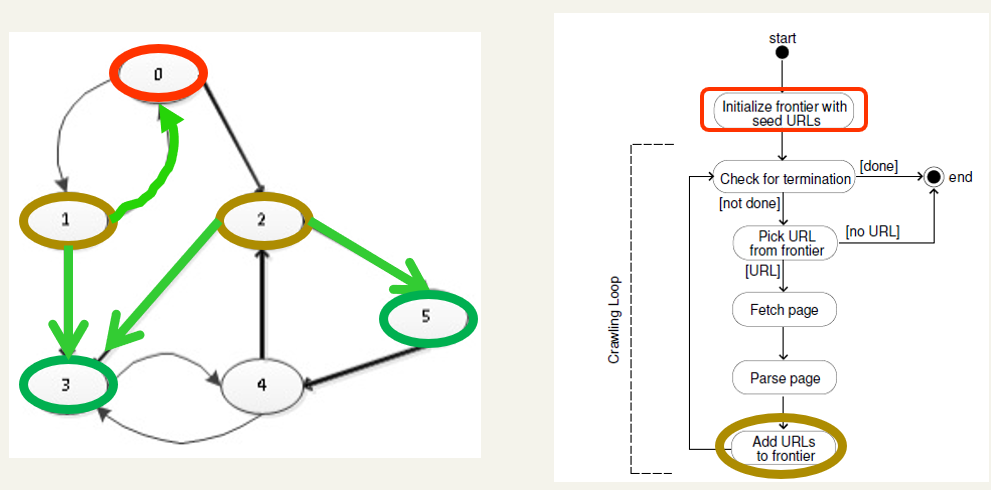
\includegraphics[width=0.75\linewidth]{images/crawlingexample.png}
    \caption{Example of crawling}
    \label{fig:crawlingexample}
\end{figure}
In this case I have just one crawler and the seed page is the node 0 and in the frontier we have "senape" nodes that are 1 and 2 from the frontier we pick the "best" node to be crawled according to the best policies that we choose. We can have many termination conditions (no other pages to crawl or time limit after that we start again from scratch). When we are in node 1 it can happen that we crawl again node 0 it depends on our design choice (freshness and frequency).\newline
Now let's look in more details the algorithm of the crawler (crawler "life cycle"). Assume for simplicity that we have just one \textbf{Crawler Manager} that it's a sort of dispatcher and extract URLs and for each of them it checks if the page has been not seen or the page has been seen, but it is an old version when one of these two cases is true it resolve the URL and assign the page to the \textbf{Assigned Repository}. Then we have one \textbf{Downloader} per page and the number of Downloader gives you the idea of parallelism that we can do. The Downloader \textbf{fetchs} the pages save them in a compressed form and assigns them to the Page Repository. At the end we have the \textbf{Link Extractor} or \textbf{Parser} (we have one of it per page) that takes pages from the Page Repository and extracts all the links in the page like href or links in javascript code and put them into the Priority Queue.\newline
In the following figure it has been shown the Crawler "life cycle" (Figure \ref{fig:lifecycle}).
\begin{figure}
    \centering
    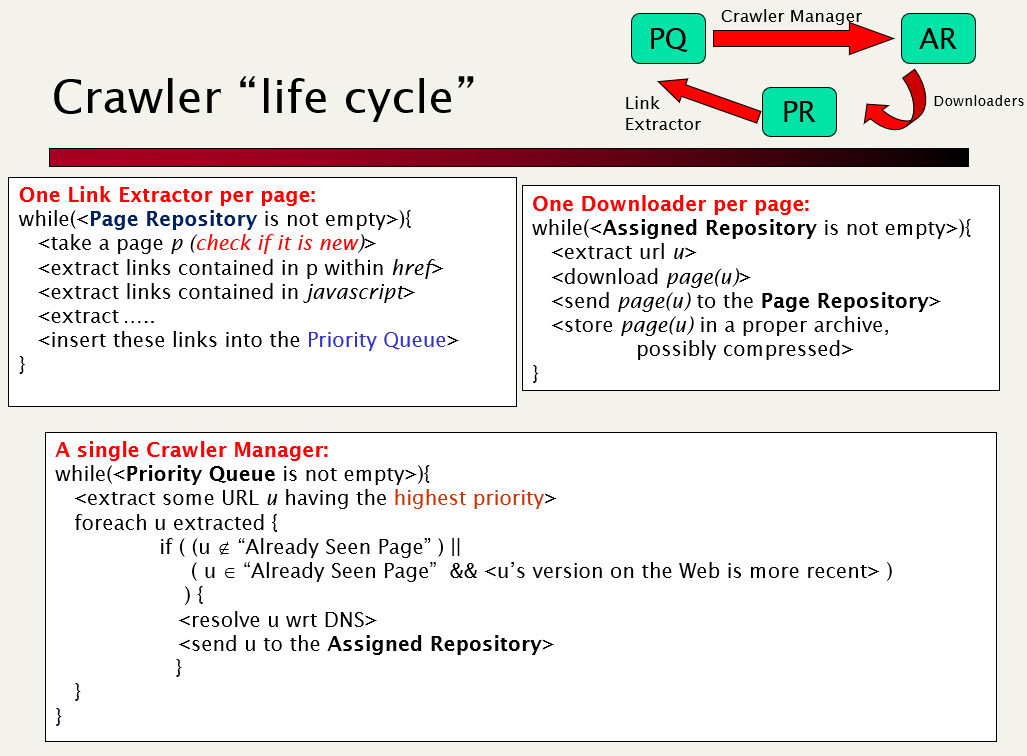
\includegraphics[width=0.75\linewidth]{images/lifecycle.png}
    \caption{Crawler "Life Cycle"}
    \label{fig:lifecycle}
\end{figure}
If we want there are a lot of open source crawlers on the web, but we need to specify just few parameters like seed pages, depth (how much deep I want to go when I enter in an host, this helps us to not enter into spider traps) and the domain of crawling. This is important to set because these crawlers are very fast and they can fill all your disk in small time.\newline
Now as we said we have the URLs frontier that has a set of pages, but given a page P, let's define how "good" P is. There are several metrics like:
\begin{itemize}
    \item BFS, DFS, Random;
    \item Popular driven where each page has a score like PageRank (obiously this is useful when you are re-crawling the Web and you already know the score of the pages otherwise if it's the first time you can't use this);
    \item Topic driven or focused crawling;
    \item Combined;
\end{itemize}
Another issue that we already talked about is: How to fast check whether the URL is new? To solve this problem we will use the Bloom Filter that it's a data sctructure that will help us with this issue.\newline
\section{The Mercator}
Now just for historical reasons we will discuss about a classic crawler that was one of the first crawlers (1999) that was used by AltaVista.\newline
In the following picture it has been shown the structure of Mercator (Figure \ref{fig:mercator}).
\begin{figure}
    \centering
    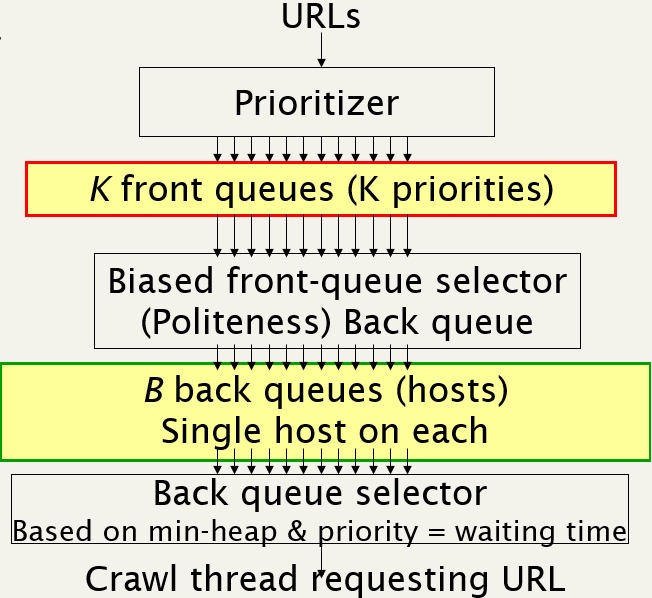
\includegraphics[width=0.75\linewidth]{images/mercator.png}
    \caption{Mercator structure}
    \label{fig:mercator}
\end{figure}
In yellow are indicated two data structures that are called queues: \textbf{K front queues} and \textbf{B back queues (hosts)} in particular they are priority queues with some features. The first one is called \textbf{Front queues} and as we already said it's a priority queue, we have K priority queues that it's a parameter that depends on the crawler. Each queue has a different priority that it's given from the \textbf{Prioritizer} and in a specific queue we can have more URLs with different domains. Then we have an algorithm that is a \textbf{selector} that picks randomly a queue from the Front queues depending on the priority (it's biased in the sense that it will pick more probably URLs from the queue K instead of the queue 1 because queue K means a larger priority than the queue 1). After this the selector put the URLs into the \textbf{Back queues} that are B, but the management of these queues is different because the distinction in the queues is done according to the host so in the same queue we will have all the URLs related to the same domain. Be careful that the crawler is able to manage only B domains. Now there is another \textbf{selector} that picks one URL from each priority queue (so we will have B URLs) and it will put them in a \textbf{min-heap} where the priority is the waiting time.\newline
Now let's go more in details with the two main parts.\newline
Starting from Front queues that manage prioritization, the prioritizer assigns to an URL an integer priority (based on refresh, quality, application specific) between 1 and K then it appends URL to corresponding queue, according to priority. In the following figure it has been shown a detailed image (Figure \ref{fig:frontqueues}).\newline
\begin{figure}
    \centering
    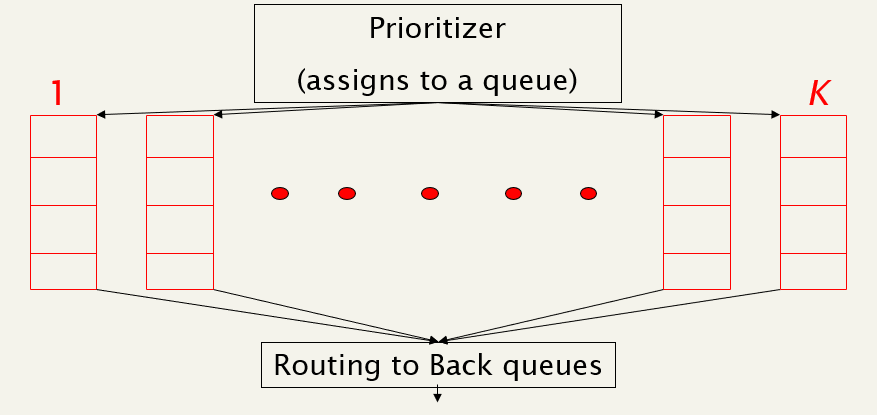
\includegraphics[width=0.75\linewidth]{images/frontqueue.png}
    \caption{Front Queues Details}
    \label{fig:frontqueues}
\end{figure}
A little bit more difficult are the Back Queues. As we said the Back Queues are B, the selector chooses a number randomly (it's biased) and goes to that queue and distributes the URLs among the B Back Queues, but there can be different problems like there is no space because either there isn't a queue with the domain of the picked URL or the queue is totally filled and I can't insert a new URL into the queue. For this reason the process of selecting URLs from the Front Queues is activated/triggered by the Back Queues when needed, we say that "Back queues enforce \textbf{politeness}" (only one connection per host is opened at time to not press to much the same host). Every queue is specialized to one single host, but host change during the running for example the i-th queue will refer to "di.unipi" then "corrieredellasera" and so on.\newline
Now what's missing is the last part, the URL selector picks from the B back queues the first item for each back queue (the queue is managed with a FIFO policy) and I insert them into the Min-Heap (with respect to some priority) that it's large B. Be careful that the priority in the Min-Heap is different from the priority that we had before because in this case it's a time interval that corresponds to the earliest time $t_e$ at which the host corresponding to the back queue can be hit again.\newline 
When we extract the min from the Min-Heap we are extracting the URL that has to be crawled first. It's advantageous to have a queue for each domain because let's suppose that we pick from the queue i-th the first item that has to be crawled at 4pm the "new" first item of that queue can't be crawled at 4pm too, but a bit later like 4.01pm.\newline
For this reason we check if the current time is larger than the time of the element in the Min-Heap we have to wait otherwise we can immediately crawl. The Heap must have always B items in particular one element for each queue.\newline
We have to discuss about a problem and is that if a back queue \textit{q} becomes empty and I ask to q a new element what happens? This means that no page from above arrived to that queue.\newline
The last part to talk about is about the crawl thread, first of all the crawl need an URL to crawl. It goes to the Min-Heap and it extracts the root of the heap (it's an URL at the head of some back queue q and then removes it). The crawlers waits the indicated time $t_{url}$. Then it parses URL and adds its out-links to the Front Queues.
Now can happen two cases when we extract an item from the back queue q:
\begin{enumerate}
    \item \textbf{The back queue q isn't empty} we pick the URL and add it to the min-heap with priority=waiting time $t_{url}$;
    \item \textbf{The back queue q gets empty} and the system doesn't have a new item to enter and it needs to fit the hole in the priority queue and for this reason it asks to the front queue to give him another URL (remember that the URL is chosen from the selector according to the priority); it can happen that the new URL is from a known host and we add it there (if the queue where we are adding it can be that the queue is full, but there is a "trick" between the size of B and K) otherwise if it's new we have a free queue that it's q and we assign the queue q to that host;
\end{enumerate}
Remember that Back Queues and Front Queues work in a \textbf{synchronized} way. A good heuristic to choose B is \textbf{B$=$(3 x threads)}.
\chapter{The Bloom Filter}
A problem that now we want to take into account is how do we fast check if a page is new or not. This problem looks trivial, but it's not because it requires time and space. We can't use an Hash Map where we put all the URLs because we crawl billion of URLs. To understand this better we can make an example let's suppose that we have 50 billion of pages (that's a small number against the real ones) and suppose that each page has 10 hyperlinks then this means that we have "seen" over 500 billion of pages. In average each URL occupies 1000 chars this means that we store 500.000 Tb (500 Pb) just to know which URLs we have already seen!\newline
At that time AltaVista used the disk access with caching, but nowadays a modern approach is the Bloom Filter that it's an archive. Supposing that we have 500 billion of URLs it occupies around 50 Tb that's very efficient.\newline
\section{Bloom Filter}
The Bloom Filter has been created in 1970 and it's a data structure that in the first times it didn't have any success, but when search engines came out it had a lot of success because was so helpful. This data structure has some good features and some bad features. First of all is good because it occupies very few space and this is important because we deal with a lot of items; on the other hand this data structure is not always "correct" that's why is called \textit{one-side error data structure} in the sense that the answer is Yes or No and if the answer is No we know for sure that it's correct, but if the answer is Yes it can be probably wrong the answer. Our goal is to estimate the probability of error (we will see that it's a low probability).\newline
Let's look at the structure of the Bloom Filter:
\begin{itemize}
    \item It's a binary array of length m, B[1,m];
    \item Consider a family of k hash functions that map a key (URL) to a position (integer) in B;
\end{itemize}
\textbf{How do we add URLs to Bloom Filter?} Whenever you have a key (URL) you compute k hash functions that will return you k positions (integer) each one of these position is set to 1 (if it's 0 we change it with 1 if it was already 1 we don't change it), this is just a binary array. In the following image it has been shown an example (Figure \ref{fig:bloomfilterexample}).


\begin{figure} [h!]
    \centering
    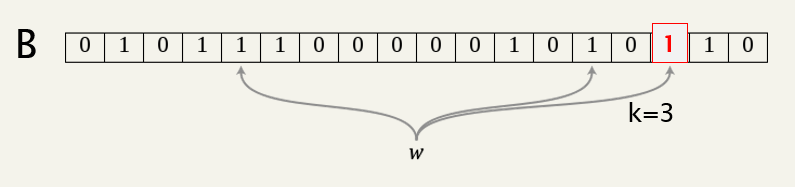
\includegraphics[width=0.75\linewidth]{images/bloomfilterexample.png}
    \caption{Bloom Filter example}
    \label{fig:bloomfilterexample}
\end{figure}
Remember that we can't delete (some positions becomes 0 where there are other URLs that go to that positions), we can just insert and get (that can be wrong for some reasons already introduced).\newline
\textbf{How do we check if an URL is already in the set?} Whenever you have a key (URL) you compute k hash functions that will return you k positions (integer) and if at least one of them is equal to 0 then I know for sure that the key wasn't in the set. Instead if when I compute the hash functions all the positions that I get are equal to 1 then the answer is \textit{maybe the URL was already in the dictionary} because these k positions could have been set to 1 by my URL or by other URLs.\newline
I don't know if the key (URL) was already in the dictionary because this data structure throws away the keys (URL) after that it insert them into the Bloom Filter. I don't store the keys because the keys are URLs and each URL requires too much space around 1000 chars one URL doing this I need to store only one array of size m. The space that I require is m bits because we have an array of size m and each cell of the array requires one bit (0 or 1). \newline
In the following image it has been shown an example of Bloom Filter in a Biology situation (Figure \ref{fig:biology}). Looking at the image the set S that shows the keys inside the Bloom Filter is thrown away that's why when I receive a new key I compute again the hash functions.
\begin{figure} 
    \centering
    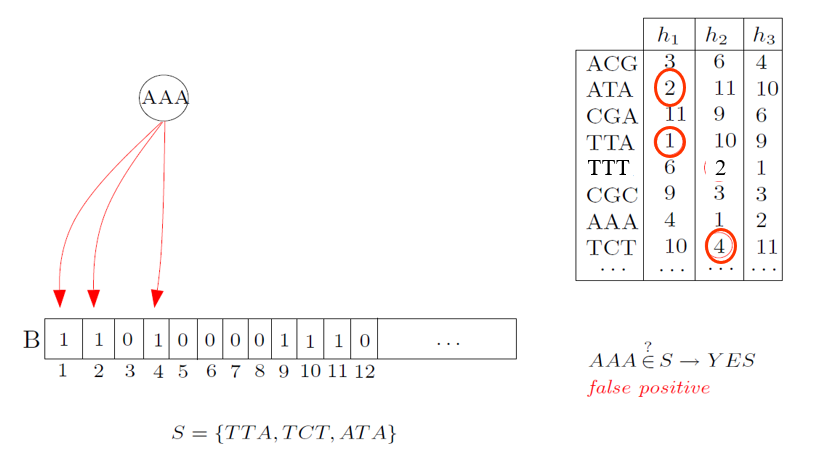
\includegraphics[width=0.75\linewidth]{images/bloomfilterbiologic.png}
    \caption{An example of Bloom Filter in Biology field.}
    \label{fig:biology}
\end{figure}\newline
\textbf{What is the probability of making an error?} The probability of making an error (\textit{false positive}) is equal to $(1-e^{-kn/m})^k$ where \textit{k} is the number of hash functions, \textit{n} is the number of the keys and \textit{m} is the size of the Bloom Filter. Furthermore it's possible to compute the minimum of this function whenever \textit{m} and \textit{n} are fixed. In fact when they are fixed we should choose $k=(m/n)ln2$ to compute the minimum we just do the derivative and set it to 0.\newline
If we put the value of k chosen following the previous rule into the formula that we have seen we obtain this:
\begin{equation}
    (1-e^{-kn/m})^k=0.62^{m/n}
\end{equation}
The size of m is larger than of n because if the array is too small I would have an array with all ones. Sometimes it's not worth to choose k like $k=(m/n)ln2$ because it can happen that $m/n$ is a large number so I would spend a lot of time checking the positions of the array (spend too time).\newline
From the previous formula we can see how if I increase the value of m then the probability of false positives goes down exponentially because m is at the exponent. Another way to understand how strong is this data structure is looking the formula from another point of view: suppose that we have $m/n=30$ I can write this as $m=30*n$ bits this means that if I use 30 bits for each key (because n is the number of keys) I can achieve a small error probability (obviously if we choose k in the best way as $k=(m/n)ln2$).\newline
If we want more into the details with the formula let's see what it happens when we choose in an appropriate way k, the \textit{general} formula becomes $(1/2)^{m*ln2/n}$ and $(0.62)^{m/n}$ comes from the fact that $(1/2)^{ln2}$ is equals to 0.62.\newline
Now let's have a fast look at the differences between the Bloom Filter and the classic Hash Table. With Bloom Filter we require a space of m bits to store n keys. Let's see what happen with the classic Hash Table, we will have a length called m' that it's proportional to n, the number of keys, $m'=\Theta(n)$ and the average list for a specific cell is $O(1)$ that it's efficient when we have to access to the list. The problem with this technique is that we must store the keys let's have a look at the space that we require. The classic Hash Table requires \textit{space of T + space of the lists}, let's go deeper with these two value. The space of T is equal to \textit{8 bytes * m'} and the space of the lists is equal to \textit{(L+8 bytes)*n} (8 bytes = space required by a pointer and L = space required by a key). Since we said that $m'=\Theta(n)$ so m' is proportional to n for simplicity assume that \textit{m'=n}. At the end we will get \textit{8n + (L+8)n} that it's equal to \textit{(L+16)n bytes}, let's transform bytes in bits to make a comparison with Bloom Filter (we must multiply by 8) \textit{(8L+128)n bits}.\newline
Let's compare the two techniques and consider the case where \textit{m < (8L+128)n}, before we said that \textit{m} should be considered bigger than \textit{n} and we can see it like \textit{n * c} (c = constant >= 1).\newline
From this we can infer that \textbf{Bloom Filter is more space efficient than HashTable iff} \textit{c < 8L+128}.\newline
At this point recall what is the error for the Bloom Filter $error=(0.62)^{m/n}$ hence $error=(0.62)^c$. \newline
The HashTable gives you always the right answer, but it occupies a lot of space instead Bloom Filter gives you an answer with a low error probability. This structure is used by some databases and virus detector.\newline
\section{Spectral Bloom Filter}
Now we are going to consider a new variation of Bloom Filter that it's able to consider counting and deletion operations that it's called Spectral Bloom Filter (SBF). The Spectral Bloom Filter is used by Search Engines because they keep into account \textit{query logs} because they want to remember the queries done by the users such that they can do statistics on queries. This variation is a dynamic data structure because it allows operations like deletion and counting.\newline
Let's show a definition of SBF \textit{M=<S, $f_x$>} is a multi-set were: S is a set and $f_x$ is a function returning the number of occurrences of x in M.\newline
There are some original features of this variation:
\begin{itemize}
    \item Space usage is slightly larger, but the performance are better;
    \item Insertions/Deletions are possible with some tricks;
    \item It manages streaming data (data that arrive after one the other and I want to manage them in the order as they arrived);
    \item It allows \textit{iceberg queries} (given x, check if $f_x > T$ dynamic threshold) and aggregate queries (SELECT count(a1) FROM R WHERE a1=v);
\end{itemize}
The B vector is replaced by a vector of counters $C_1$, $C_2$, ..., $C_m$ and $C_i$ is the sum of $f_x$ values for elements $x \in S$ mapping to i. This means that the approximations of $f_x$ are stored into $C_{h_1(x)}$, $C_{h_2(x)}$, ..., $C_{h_k(x)}$. Since we can have conflicts in the same cell the $C_i$ provides approximations.\newline
In the following figure it has been shown an example (Figure \ref{fig:minimumselection}).
\begin{figure}
    \centering
    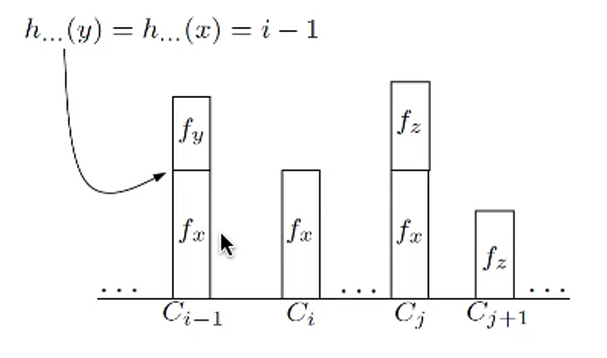
\includegraphics[width=0.75\linewidth]{images/minimumselection.png}
    \caption{Example of Spectral Bloom Filter}
    \label{fig:minimumselection}
\end{figure}
From the image we can see:
\begin{itemize}
    \item $C_{i-1}$ is not a good approximation of $f_x$ (neither of $f_y$) because I had a collision;
    \item $C_i$ is an exact approximation of $f_x$;
    \item $C_{j+1}$ is an exact approximation of $f_z$;
\end{itemize}
Obviously I would like to not have collision such that the cell dedicated to a specific item gives me the exact number of occurrences. Let's highlight that I can have only overestimation, I can't have underestimation because I just sum items. I hope that when the k hash functions give me k positions at least one of them is correct and that's why I always take the minimum (it's clear that it's not always correct).\newline
Let's see in more details the algorithms of \textit{insertion} \textit{deletion} and \textit{search}.
\begin{itemize}
    \item The insertion is simple because what we do is just for each hash function we compute the position and we increase by 1 that position;
    \item The deletion is simple too because it's like the insertion, but instead of summing we decrease each counter by 1; we assume that we do deletion only of things that we already have we can't delete things that we don't have;
    \item Searching for an element x needs to compute the positions for all the hash functions and then return the \textbf{Minimum Selection} (MS) value between all the values that I got;
\end{itemize}
Notice that in this case each cell has counter instead of just one bit so we should choose how many bits assign to them. For example if we choose 5 bits then it means that we can represent at most $2^5$ counters.\newline
\textbf{How can we prove that the Spectral Bloom Filter has the same error of Bloom Filter?} Let's reason on this, the probability of have an error is the probability that all the cells that I check have a collision, but this is exactly the error probability of the Bloom Filter (it fails when all the cells that I check are ones and the key is not in the set). The error is the same as for Bloom Filters.\newline
\textbf{Theorem:} For all \textit{x}, it is $f_x <= m_x$. Furthermore $f_x != m_x$ with probability $E_{SBF}= \varepsilon \approx (1-p)^k$. (Here the formula is the same as Bloom Filter, but the value \textit{m} is the number of cells and not the number of bits).\newline
\textbf{Proof:}
\begin{itemize}
    \item The case $m_x < f_x$ cannot happen;
    \item The event $m_x > f_x$ is "all counter $C_{h_i(x)}$ have a collision", that corresponds to a "false positive" event of classical BF;
\end{itemize} 
We have mainly two challenges to improve:
\begin{enumerate}
    \item allow insertion/deletion keeping low $E_{SBF}$;
    \item dynamic array of variable-length counters (suppose that I'm using a lot of bits for each cell and in one cell I have counter equals to 1, I'm wasting space), but we will not see how to manage this problem;
\end{enumerate}
To solve the first problem we introduce the idea of \textbf{Recurring Minimum} (RM). To better understand this concept let's have a look at this simple figure (Figure \ref{fig:recurringminima}).
\begin{figure}
    \centering
    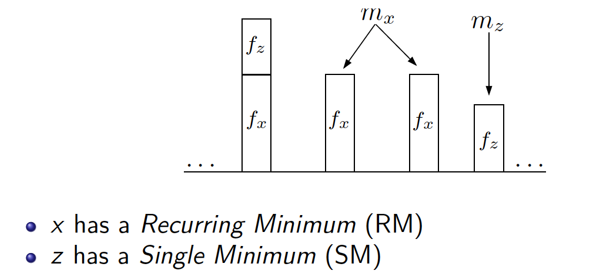
\includegraphics[width=0.75\linewidth]{images/recurringminima.png}
    \caption{Example of Recurring Minimum}
    \label{fig:recurringminima}
\end{figure}
Let's give a definition of Recurring Minimum (RM): an element has a RM iff more than one of its counters has value equal to the minimum. The idea is that if we have a RM it's very improbable that the value it's wrong because it means that there are other items that accessed to that positions and increased always the same positions.\newline
Instead if the minimum recurs just one time then it's called \textbf{Single Minimum} (SM). In general the algorithm says that if we have a RM we consider that value as our result, but if we have a SM we do other stuff because we aren't sure about that result.\newline
\textit{Basic idea:} We operate as in MS (Minimum selection), but over two SBF.
\begin{enumerate}
    \item For item x with RM we use $m_x$ as estimator which is highly probable to be correct: hence $E_{SBF_1} < \varepsilon$ (because the minimum occurs more times than one time);
    \item For item with a SM we use a secondary SBF which is $|SBF_2| \ll |SBF_1|$ and thus can guarantee $E_{SBF_2} \ll \varepsilon$;
\end{enumerate}
We use more space which could be used for enlarging the single BF, but it has been shown that improvements may be remarkable that's why we use this variation!\newline
Now let's analyze how we do operations with Recurring Minimum.\newline
\textbf{Insertion}: first of all we increase all the counters of x in $SBF_1$ then we check if x has a RM in $SBF_1$ we stop otherwise we go to $SBF_2$ and we look for x; now we can have two cases: the first one is that x is already in $SBF_2$ and we only need to increase by 1 all the counters otherwise we set x in $SBF_2$ as the minimum value of x in $SBF_1$ (we increase using the minimum so the cells equal to 0 become equal to the minimum and the cells different from 0 are increased using the minimum for example if we have 0 and 1 and the minimum is 3 then we get 3 and 4).\newline
\textbf{Deletion}: is the inverse of the insertion so first of all we decrease all the counters of the $SBF_1$ then we check if x has a SM in $SBF_1$ if this is true then we go to the $SBF_2$ and we decrease all the counters of x in $SBF_2$ (if any).\newline
\textbf{Lookup/Search}: first of all I check the value of x in $SBF_1$ and if I have a RM I can stop otherwise if I have a SM I go to the $SBF_2$ and I check if the value of x is greater than 0 I take it as a result otherwise I take as result the minimum of the $SBF_1$.\newline
In the following image it has been shown the pseudo-code of these three operations with SBF with RM (Figure \ref{fig:insdelloo}).\newline
\begin{figure}
    \centering
    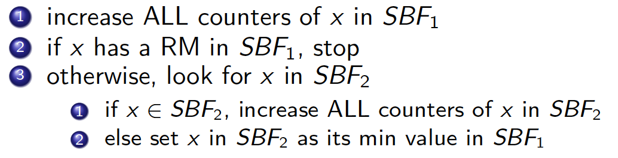
\includegraphics[width=0.75\linewidth]{images/insertion.png}
    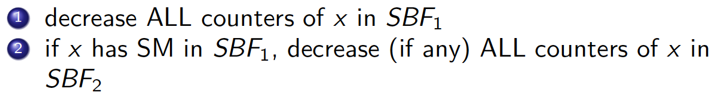
\includegraphics[width=0.75\linewidth]{images/deletion.png}
    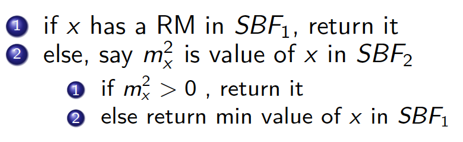
\includegraphics[width=0.75\linewidth]{images/lookup.png}
    \caption{Pseudo-code of insertion, deletion and lookup}
    \label{fig:insdelloo}
\end{figure}
\textbf{Notice} that if we know a prior all the dictionary of items we can avoid the problem, that a key from a RM become a SM inserting a new key, this never occurs. To avoid this we can initialize the structure inserting all the keys with value 1 only in the First SBF such that we surely have all the keys present and then we start counting. It never occurs that a new key arrives and destroys a RM that we had before. If this occurs the key was already present before so the clashing cell was already identified as a "colliding" cell. Obviously we can do this only when we already have all the dictionary.\newline
\chapter{Parallel Crawlers}
In this chapter we will discuss about a problem that it's how to distribute the work among different crawlers that work in parallel for example how we have to assign tasks to the downloaders that will download pages.\newline
In order to make this process efficient we have to avoid the duplication of work in the sense that whenever some pages have to be crawled they must be assigned only to one single bot/crawler/spider.\newline
There are two approaches to solve this problem:
\begin{itemize}
    \item \textbf{Static assignment:} this is the simplest assignment and suppose that for some reason we are able to partition the web and we assign each part of the web to a specific crawler; the goal is to have a balance partition s.t. each crawler has the same amount of work to do; obviously we can't assign to each crawler a specific domain because each domain has different size (".it" is smaller than ".com"); ideally this would be nice, but it's not affordable;
    \item \textbf{Dynamic assignment:} this is something where we have a coordinator that leads the crawler and it distributes URLs to the crawlers trying to keep balanced the work; in this case to guarantee that the work is balanced we can use an hash function \textit{h} that takes an URL and returns as output a number that it's in the range between [0, c-1] (this is simple to be build) where \textit{c} is the number of the crawlers/downloaders; that's it if the hash function is sufficient good taken a set of URLs it will distribute them in a balanced way the URLs between all the crawlers;
\end{itemize}
As we said we have these two approaches, but the best one that it's used is the dynamic assignment. Now let's have a look at what can happen.\newline
\textbf{How do we manage fault-tolerance} because if a crawler dies or a new crawler is added we need to recompute again an hash function and all the URLs have to be assigned again. To solve this problem there is a solution that it's called \textbf{Consistent Hashing}.
\section{Consistent Hashing}
This solution has been proposed by an MIT group, the same that created Akamai the largest content delivery network, but now let's look at the idea.\newline
Assume to consider a space like a ring with integer numbers from [0, $2^k-1$] (to implement this we can just use modulo and we get it). Now you can have one hash function or more hash functions. For simplicity we can consider just one hash function and the domain is $U$ (space of the objects that I want to distribute so they are servers/crawlers or items/URLs) and the co-domain is the ring so [0, $2^k-1$] so this means that the hash function is in modulo $2^k$.\newline
Assume that you have a set of servers $s_1$, $s_2$, ..., $s_n$ to map then we take the hash function and we apply it to all the server getting $h(s_1)$, $h(s_2)$, ..., $h(s_n)$. These values are integers in particular they are positions of the ring. This is the first distribution and it's totally random. Now we do the same thing with my items $u_1$, $u_2$, ..., $u_m$ and we will get as result $h(u_1)$, $h(u_2)$, ..., $h(u_m)$ that are always integers in particular they are positions of the ring.\newline
Notice that it can happen that the same position is assigned to a server and to an url.\newline
The question now is \textbf{how do we map URLs to servers?} we just need to take the ring and read it clock-wise or anti clock-wise and assume that we choose it clock-wise we will have that \textit{all the URLs that occur before the server $s_i$ will be assigned to it up to the first server that we meet}, in other words we can imagine the server as the head of this list.\newline
This is the idea, but the question is \textit{why is this advantageous?} Suppose that one machine is broken then we don't have to remap all the objects, like the previous solution, but we have to remap only the objects assigned to that machine and to do that we just add them to the \textit{tail} of the next server.\newline
On average if \textit{n} is the number of the URLs and \textit{s} is the number of the servers then $n/s$ will be the \textbf{average number of items assigned to one server}. So if one server is broken we have to remap only $n/s$ objects instead of n.\newline
\textbf{What happens if I add a new server?} It's exactly the same because I put the new server in the middle of a trail and I will "split up" the number of items assigned to the previous server. We can see insertion as a "split" and deletion as a "merge".\newline
There is a property that can be proved about \textit{sampling} if you want guarantee that $n/s$ is the right distribution of objects instead of sampling s objects you sample $s*log(s)$ and then among these $s*log(s)$ you pick just one over s; in other words you map the server on the ring and then the distance between two servers is log(s) thanks to this we are guaranteeing that the distribution is more concentrated over $n/s$ (each server gets replicated log s times).\newline
\section{Software Crawlers}
There are some open source software to crawl the web like Nutch from Apache Foundation or Scrapy that it's written in Python (from this it comes the suffix "py"). To use these software you just need to specify which are the seeds (starting page) and the bounds (the domain) and at the end you can specify the level, how deep you want to go. Usually it's recommended to keep the level <= 2 that allows you to crawl a lot of pages otherwise the disk can be filled in few time.